\documentclass{standalone}

\usepackage{tikz}
\usetikzlibrary[folding] 
\begin{document}
	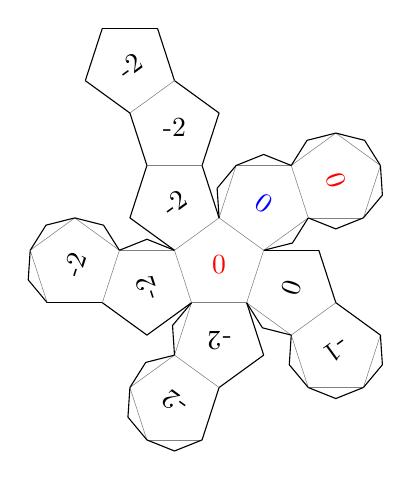
\begin{tikzpicture}[transform shape]
	\tikzfoldingdodecahedron
	[folding line length=7mm,
	face 1={ \node[red]{0};},
	face 2={ \node[blue] {0};},
	face 3={ \node[red]{0};},
	face 4={\node {0};},
	face 5={ \node {-1};},
	face 6={ \node{-2};},
	face 7={ \node{-2};},
	face 8={ \node{-2};},
	face 9={ \node{-2};},
	face 10={ \node{-2};},
	face 11={ \node{-2};},
	face 12={ \node{-2};}
	];
	\end{tikzpicture}
\end{document}